\chapter[2025 July]{July 2025}

\section[2025/07/05]{Friday, 4 July 2025}
\label{sec:20250704}

Considering the old approach didn't work (no reason in reconstructing the nodes) the new approach is as follows:

\subsection{Problem Formulation}

Given an image $I$ containing $P$ people, where each person $p$ has a set of
detected joints $J_p = \{j_{p,1}, j_{p,2}, \ldots, j_{p,K}\}$ with $K=17$
keypoints (COCO format), the goal is just to learn a function that groups joints by
person identity.

Each joint $j_{i}$ is represented as:
\begin{equation}
\label{eq:joint_representation}
j_i = [x_i, y_i, d_i, c_i, \mathbf{e}_i] \in \mathbb{R}^{4+D}
\end{equation}

where $(x_i, y_i)$ are 2D coordinates, $d_i$ is estimated depth, $c_i$ is
confidence score, and $\mathbf{e}_i \in \mathbb{R}^D$ is a learnable joint-type
embedding.

\subsection{Mixed Graph Construction}

For each image, construct a single graph $G = (V, E)$ where:

\begin{align}
V &= \bigcup_{p=1}^{P} J_p = \{j_1, j_2, \ldots, j_N\} \\
E &= \emptyset \quad \text{(no initial edges)}
\end{align}

Each node $v_i \in V$ has associated ground truth person label $y_i \in \{1, 2, \ldots, P\}$.

\subsection{Graph Attention Network Architecture}

The model consists of two GAT layers followed by a pairwise classifier:

\subsubsection{Feature Embedding}
\begin{align}
\mathbf{h}_i^{(0)} &= j_i \in \mathbb{R}^{4+D} \\
\mathbf{h}_i^{(1)} &= \text{GAT}_1(\mathbf{h}_i^{(0)}, \mathcal{N}(i)) \\
\mathbf{h}_i^{(2)} &= \text{GAT}_2(\mathbf{h}_i^{(1)}, \mathcal{N}(i))
\end{align}

where $\mathcal{N}(i)$ represents the attention-based neighborhood of node $i$, and $\mathbf{h}_i^{(2)} \in \mathbb{R}^{d_{embed}}$ is the final joint embedding.

\subsubsection{Pairwise Classification}
For any pair of joints $(i,j)$, compute:
\begin{align}
\mathbf{z}_{ij} &= [\mathbf{h}_i^{(2)} \parallel \mathbf{h}_j^{(2)}] \in \mathbb{R}^{2d_{embed}} \\
s_{ij} &= \text{MLP}(\mathbf{z}_{ij}) \in \mathbb{R} \\
p_{ij} &= \sigma(s_{ij})
\end{align}

where $\parallel$ denotes concatenation, $\text{MLP}$ is a multi-layer
perceptron, and $p_{ij}$ represents the probability that joints $i$ and $j$
belong to the same person.

\subsection{Training Objective}

\subsubsection{Pairwise Label Generation}
For each training graph, generate pairwise labels:
\begin{equation}
\ell_{ij} = \begin{cases}
1 & \text{if } y_i = y_j \text{ (same person)} \\
0 & \text{if } y_i \neq y_j \text{ (different people)}
\end{cases}
\end{equation}

\subsubsection{Loss Function}
The training objective is binary cross-entropy over all pairs:
\begin{equation}
\mathcal{L} = -\frac{1}{|\mathcal{P}|} \sum_{(i,j) \in \mathcal{P}} \left[ \ell_{ij} \log p_{ij} + (1-\ell_{ij}) \log(1-p_{ij}) \right]
\end{equation}

where $\mathcal{P} = \{(i,j) : i < j, i,j \in V\}$ is the set of all joint pairs.

\subsection{Inference Pipeline}

At inference time, given a new image with detected joints:

\begin{enumerate}
\item \textbf{Feature Extraction}: Compute joint embeddings $\{\mathbf{h}_i^{(2)}\}_{i=1}^N$
\item \textbf{Pairwise Prediction}: For all pairs $(i,j)$, compute $p_{ij}$
\item \textbf{Graph Construction}: Create adjacency matrix $A$ where $A_{ij} = 1$ if $p_{ij} > \tau$ (threshold)
\item \textbf{Connected Components}: Find connected components in graph $(V, A)$ to group joints by person
\end{enumerate}

\subsection{Key Advantages}

\begin{itemize}
\item \textbf{Direct Optimization}: Loss function directly optimizes grouping performance
\item \textbf{Realistic Training}: Mixed graphs simulate inference conditions with multiple people
\item \textbf{No Structural Assumptions}: No predefined skeletal connections required
\item \textbf{Scalable}: Handles variable numbers of people without hyperparameter tuning
\item \textbf{Interpretable}: Pairwise predictions provide insight into model decisions
\end{itemize}

\subsection{Implementation Details}

\begin{itemize}
\item Joint embeddings: $D = 32$ dimensional learnable embeddings for 17 keypoint types
\item GAT architecture: 4 attention heads, hidden dimension 64, output dimension 32
\item Pairwise MLP: [64, 32, 1] with ReLU activations and dropout (0.6)
\item Optimization: Adam optimizer with learning rate $10^{-3}$
\item Training: Binary cross-entropy loss, batch size 8 graphs
\end{itemize}

did a run with this one basic\_v2

it terminated with the following error so fix that later

\begin{lstlisting}[style=,title={Error to fix later on basic v2},label={code:basic_v2_error}]
Exception has occurred: ValueError
Target size (torch.Size([1])) must be the same as input size (torch.Size([]))
  File "/home/dean/projects/mills_ds/code/pipeline/basic_v2/trainer.py", line 72, in train
    loss = F.binary_cross_entropy_with_logits(pair_predictions, pair_labels.float())
           ^^^^^^^^^^^^^^^^^^^^^^^^^^^^^^^^^^^^^^^^^^^^^^^^^^^^^^^^^^^^^^^^^^^^^^^^^
  File "/home/dean/projects/mills_ds/code/pipeline/main.py", line 171, in main
    dataset=processed_train_graphs,

        epochs=num_epochs,

        batch_size=batch_size_trainer,

        lr=learning_rate

    )
          ^^^^^^^^^^^^^^^^^^^^^^^^^^^^^^^^^^^^^^^^^^^^^^^^^^^^^^^^^^^^^^^^^^^^^^^^^^^^^^^^^^^^^^^^^^^^^^^^^^^^^^^^^^^^^^^^^^^^^^^^
  File "/home/dean/projects/mills_ds/code/pipeline/main.py", line 197, in <module>
    main()
ValueError: Target size (torch.Size([1])) must be the same as input size (torch.Size([]))
\end{lstlisting}

I have some results 

\begin{figure}[H]
	\centering
	
\includegraphics[width=0.4\linewidth]{figures/training_attempt_3/embeddings_epoch_50.png}
	
\includegraphics[width=0.4\linewidth]{figures/training_attempt_3/embeddings_epoch_100.png}
	
\includegraphics[width=0.4\linewidth]{figures/training_attempt_3/embeddings_epoch_150.png}
	
\includegraphics[width=0.4\linewidth]{figures/training_attempt_3/embeddings_epoch_200.png}
	
\includegraphics[width=0.4\linewidth]{figures/training_attempt_3/embeddings_epoch_250.png}
	\caption{Training with full set and 250 epochs reconstruction}
	\label{fig:training_attempt_3_embeddings_epocs}
\end{figure}

\begin{figure}[H]
	\centering
	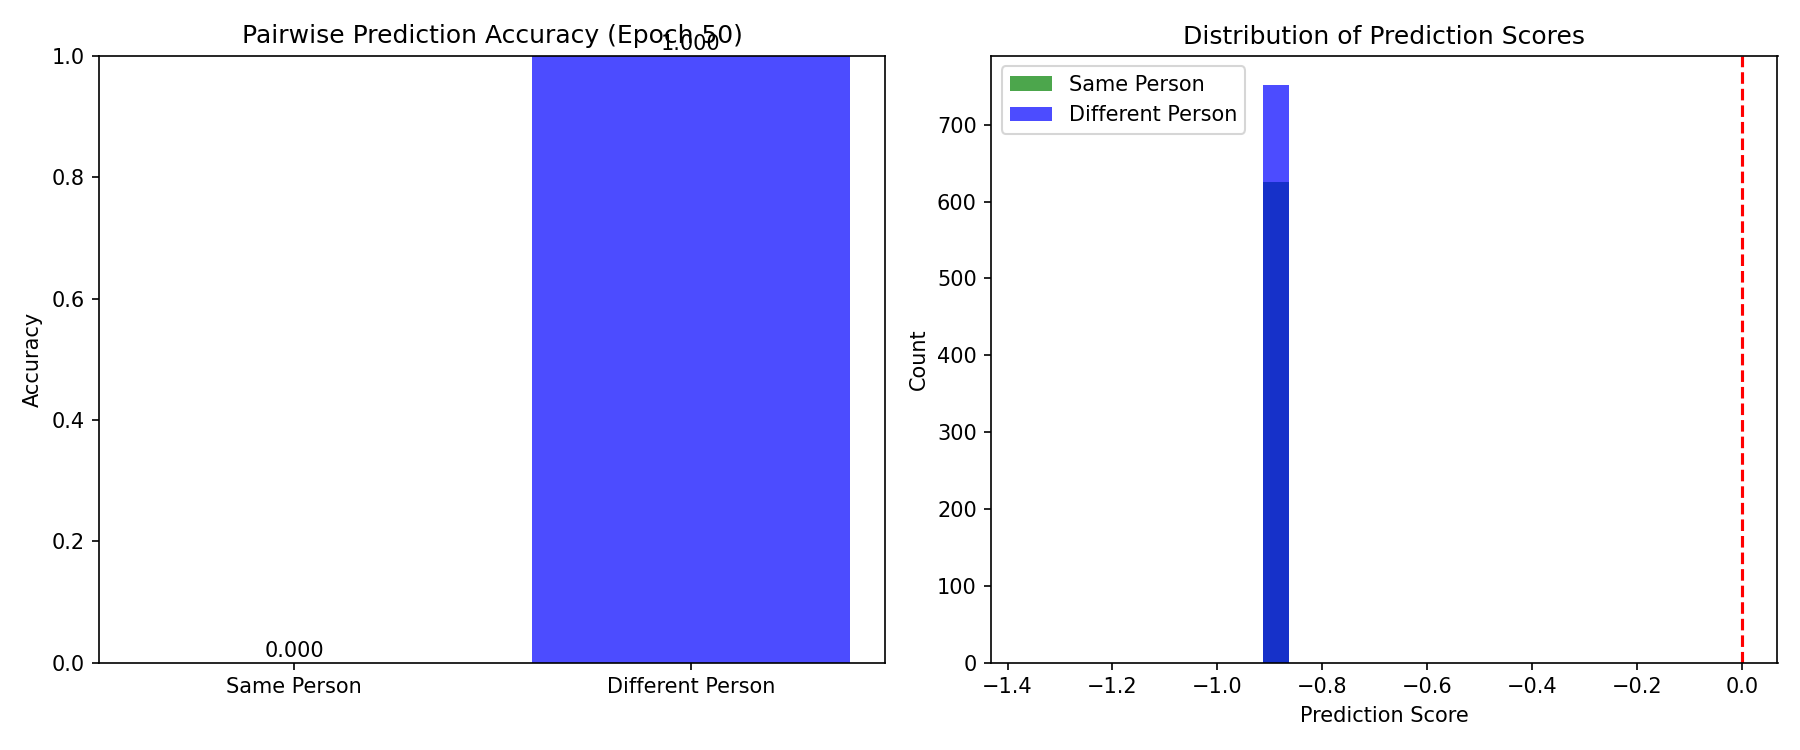
\includegraphics[width=0.4\linewidth]{figures/training_attempt_3/pairwise_epoch_50.png}
	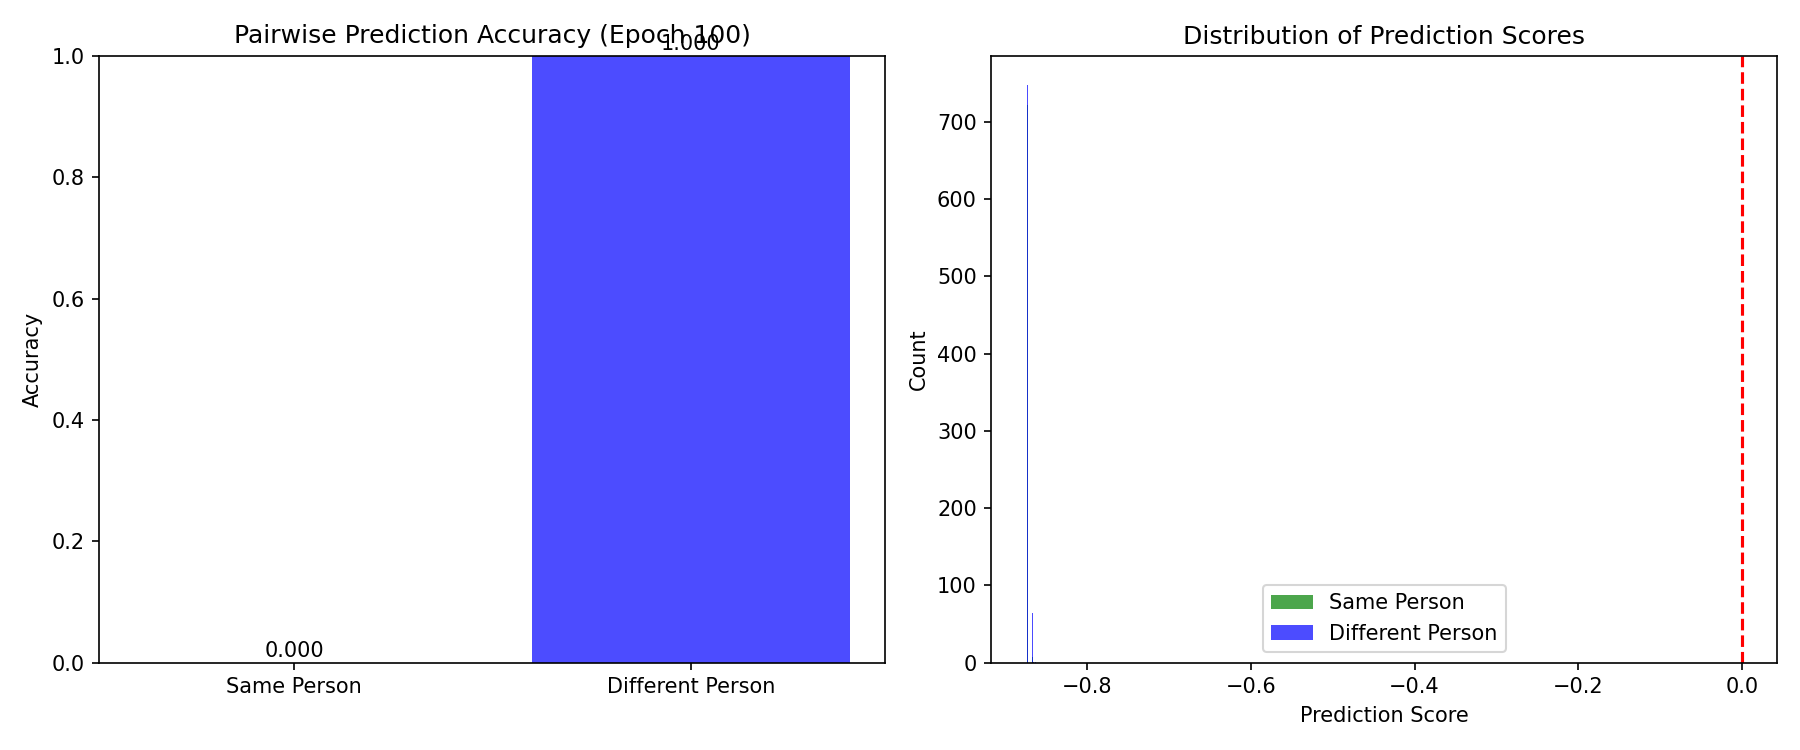
\includegraphics[width=0.4\linewidth]{figures/training_attempt_3/pairwise_epoch_100.png}
	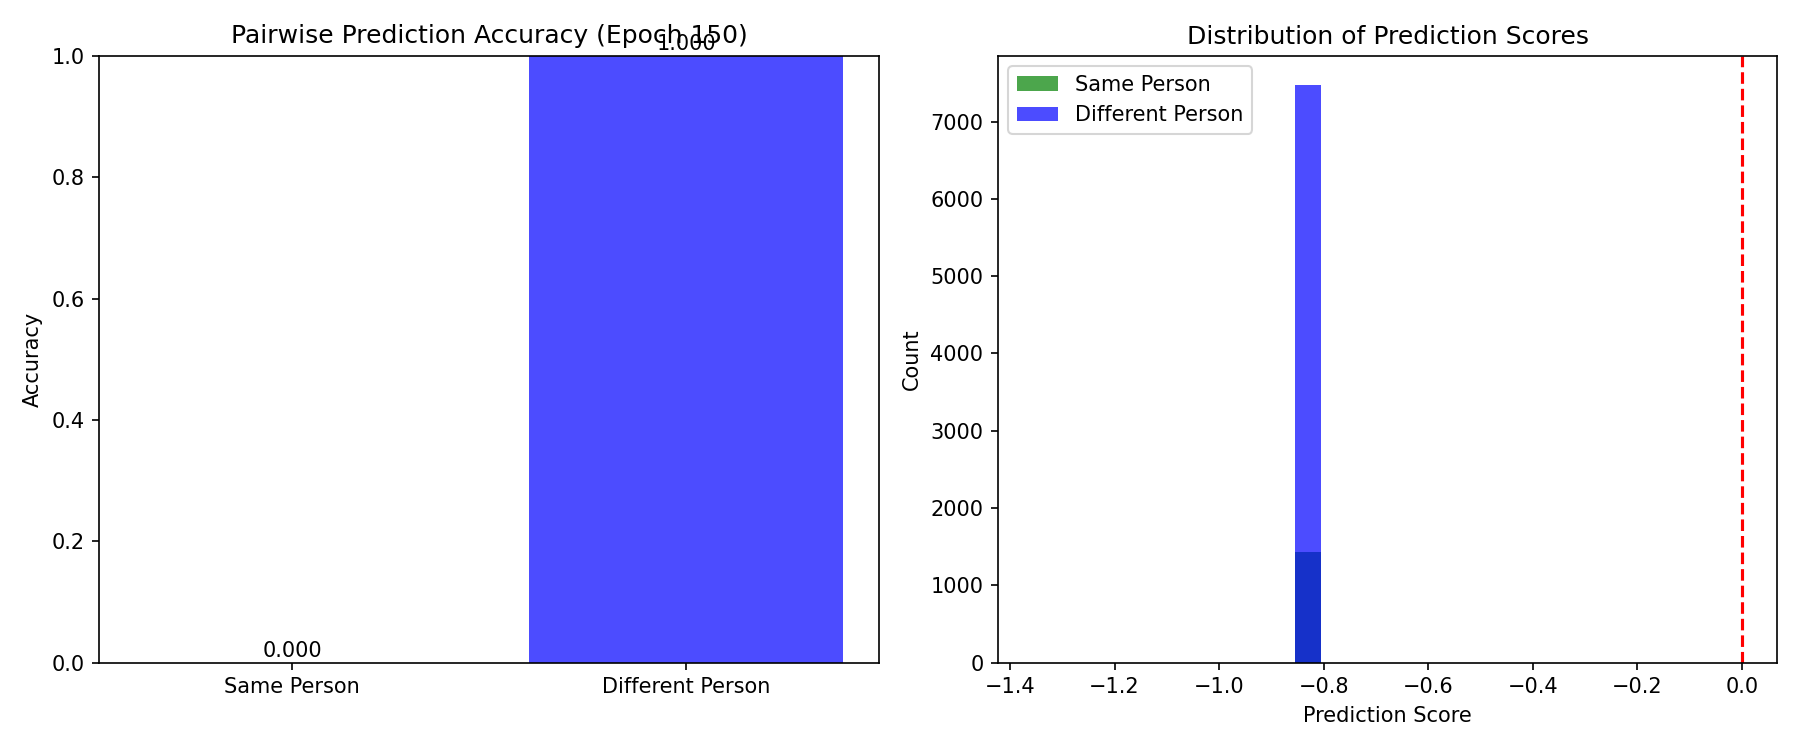
\includegraphics[width=0.4\linewidth]{figures/training_attempt_3/pairwise_epoch_150.png}
	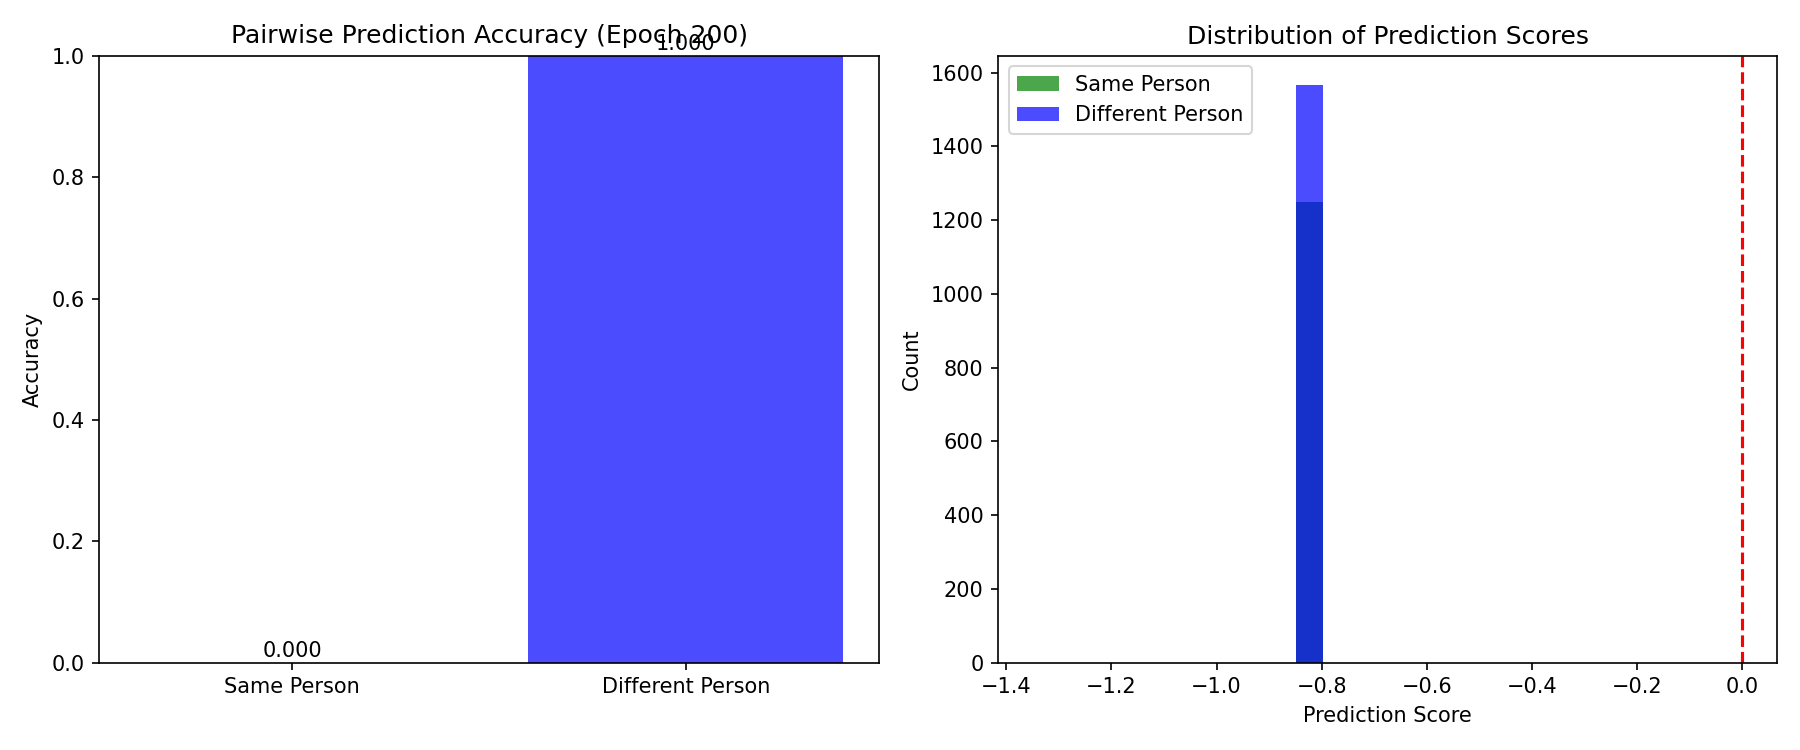
\includegraphics[width=0.4\linewidth]{figures/training_attempt_3/pairwise_epoch_200.png}
	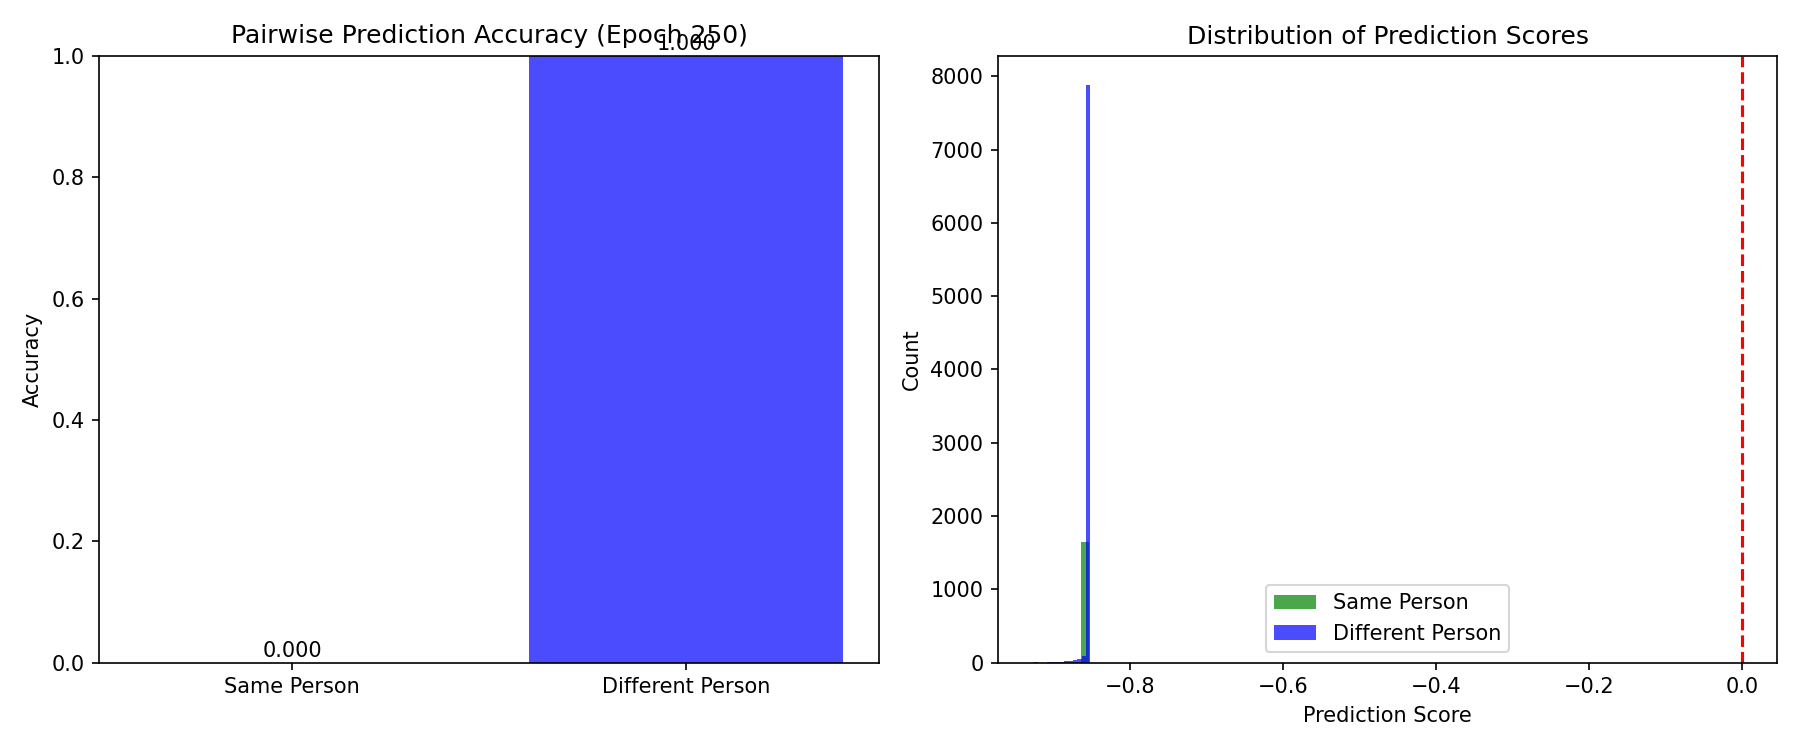
\includegraphics[width=0.4\linewidth]{figures/training_attempt_3/pairwise_epoch_250.png}
	\caption{Training with full set and 250 pairwise prediction accuracy}
	\label{fig:training_attempt_3_pairwise_epocs}
\end{figure}

\section[2025/07/17]{Thursday, 17 July 2025}
\label{sec:20250717}

There are a couple problems here. The issue is that I don't know if this is working and how to approach it

The loading of the data is a massive bottle neck

I'm going to use better versioning so that I don't have to include code in this document.

I tried to cache the dataset (val worked but training didn't it crashed my computer)

\subsection{Issue}

The issue here is that I don't really know how this works internally but I'm just trying to implement 
different approaches. The pairwise approach above seemed reasonable but I don't think it will work.
It treats keypoints groupings as a binary classification problem: so for every pair of keypoints,
predict whether they belong to the same person (1/True) or not (0/False).

Now if you take all keypoints from an image and create all possible pairs (not using the skeletal structure)
for n keypoints $\frac{n\times(n-1)}{2}$ pairs (I think) so it scales quadratically but obviously you'd 
use the skeletal structure and only make realistic pairs. With this being said you still need to create a lot
of connections and rules about those so using the model you'll know left wrist to left elbow but then maybe
symmetry as well so left shoulder to right shoulder.

Think for the simple implementation I'm going to try just learn person\_id directly

\subsection{Node Features}

I think the simplest node feature I should create is [x,y,depth,confidence, joint\_type] here are some questions:

\begin{compactitem}
	\item normalize x,y by dividing by image width/height?
	\item how should I normalize depth? 
	\item how can I relate these two things to each other? 
	\item the confidence should I just keep 0,1,2 or use a probability
\end{compactitem}

For a first approach which I'm trying to do here leave everything as is (raw) and let the gat figure it out.
Then start normalizing and see if that improves training.

Node Features = [raw x, raw y, raw depth, raw confidence, joint type]

The joint type can either just be an index likes 0,1,2,... etc or maybe 1 hot encoded vector like 1,0,0,0 for 0 and 0,1,0,0 for 1 and so on

\subsection{Depth estimation}

Going to keep using midas for this seems to be working well

\subsection{Preprocessing}

The preprocessing simplification still requires a mixed graph 

Input:

\begin{compactitem}
	\item image (tensor [C,H,W]) 
	\item keypoint\_list
\end{compactitem}

where keypoint\_list is [person\_0\_keypoints,person\_1\_keypoints,...] and each person keypoints is [17,3] which is 17 keypoints with [x,y,confidence]

the processing flow is as follows

\begin{compactitem}
	\item estimate depth for image 
	\item loop through every person then every keypoint 
		\begin{compactitem}
			\item get x,y and confidence
			\item loop up depth using x,y
			\item create node feature
			\item track which person keypoint belongs to
		\end{compactitem}
	\item stack all nodes into a graph
\end{compactitem}

Output:

A single PyG Data object where:

Nodes: all keypoints from all people in the image

person\_labels: [0,0,0,...,1,1,1,...,n,n,n] (which person each node belongs to)

example:

Input: Image with 2 people

Person\_0: nose, left\_shoulder, right\_shoulder 

Person\_1: nose, left\_eye 

Output:

\begin{compactitem}
	\item 5 nodes total 
	\item person\_labels = [0,0,0,1,1] 
\end{compactitem}

The PyG Data object is a way of representing a single graph (container)

x (node features), edge\_index (graph connections) and custom attributes

x (node features):

\begin{compactitem}
	\item shape: [num\_nodes, num\_features] 
	\item each row is a one nodes features 
	\item in this case [x,y,depth,confidence,joint\_type]
\end{compactitem}

edge\_index: 

\begin{compactitem}
	\item shape: [2, num\_edges] 
	\item each column represents one edge so source and targe node 
\end{compactitem}

\begin{lstlisting}[style=pythonstyle,title={PyG edges example},label={code:pyg_edges_example}]
edge_index = torch.tensor([
    [0, 1, 2],  # source nodes
    [1, 2, 0]   # target nodes  
])
\end{lstlisting}

represents 3 edges

\begin{compactitem}
	\item Edge 1: node 0 to node 1 
	\item Edge 2: node 1 to node 2 
	\item Edge 3: node 2 to node 0
\end{compactitem}

assuming a simple example with 2 people and 3 keypoints

\begin{lstlisting}[style=pythonstyle,title={PyG Data model simple example},label={code:pyg_simple_example}]
data = Data(
    x=torch.tensor([
        [100, 150, 0.5, 1.0, 0],  # person 0, nose
        [90,  180, 0.6, 1.0, 5],  # person 0, left shoulder  
        [200, 160, 0.4, 1.0, 0],  # person 1, nose
    ]),
    edge_index=torch.tensor([[0, 1],
									 [1, 0]]),  # connect nodes 0 and 1
    person_labels=torch.tensor([0, 0, 1]),      # ground truth labels
    num_people=2
)
\end{lstlisting}

but anyways in our example just going to set the edge\_indexs to an empty tensor (no connections)
and hopefully let it figure out what the connections are meant to be

Made a basic version of this and tested seems to be working but yeah not sure about the 0 connections

\subsection{GAT}

Now the issue is that you can't just predict person ids directly because what does that even mean.
The PyG Data object knows about person id 1,2,..,n but what can it do with this information.
The idea is to use embeddings where keypoints from the same person are close together in embeddings space
and then group them.

Training:

\begin{compactitem}
	\item Input: Graph with all keypoints (from the image) 
	\item Each keypoint gets an embedding vector 
\end{compactitem}

Training goal is if keypoint A and B belong to the same person MINIMIZE the distance between embeddings
and if keypoint A and C belong to different people MAXIMIZE the distance between embeddings

Loss Function (Contrastive Learning)

\todoredefined{check the loss function not sure exactly about it}

\begin{compactitem}
	\item Positive pairs: Keypoints from same person minimize 
	\item Negative pairs: Keypoints from different person maximize 
\end{compactitem}

Inference:

\begin{compactitem}
	\item Get embeddings 
	\item Cluster (K-Means or DBSCAN)
	\item Each cluster is a person
\end{compactitem}

The details of this simple implementation is as follows

\begin{lstlisting}[style=pythonstyle,title={Simple GAT Init},label={code:pyg_simple_gat_init}]
def __init__(self, input_dim=5, hidden_dim=32, output_dim=16, num_heads=2, dropout=0.1):
\end{lstlisting}

input dim is 5 because of the node features [x,y,depth,confidence,joint type]

output dim is 16 so representing each node with a 16 dimensional embedding vector for clustering later

hidden dim is 32 (intermediate layer between input and output) 5 -> 32 -> 16

number heads is 2 (this is the number of attention heads in the first layer) as you increase the number of heads the model can pay
attention to more things (aspects)

Example:

Input: $[100.5, 200.3, 0.8, 1.0, 5]$ (one keypoint/one node)

Output: $[0.2, -0.1, 0.8, 0.3, -0.5, ..., 0.1]$ (some arbitrary 16 dimensional embedding)

Then extending this to a full graph 

Input: $[N, 5]$ where N is the number of keypoints 

Output: $[N,16]$ (each row an embedding)

so 20 keypoints is 20 embeddings of 16

\subsection{Trainer}

The goal is to train the GAT to learn embeddings where keypoints from the same person are close together and different people far
apart in embedding space.

The concept of contrastive loss (and again this seems right but I'm not sure)

For same person pair pull embeddings closer (minimize distance)

For different person push their embeddings apart (maximize which is done with a margin) 

\begin{lstlisting}[style=pythonstyle,title={Simple GAT Contrastive loss},label={code:pyg_simple_gat_contrastive_loss}]
if same_person:
    loss = distance  # Want this to be small
else:
    loss = max(0, margin - distance)  # Want distance > margin
\end{lstlisting}

Training loop:

\begin{compactitem}
	\item Get batch 
	\item Process into graphs (using the preprocessor) 
	\item For every graph 
		\begin{compactitem}
			\item forward pass (get embeddings) 
			\item create all pairs of keypoints 
			\item calculate distances between embeddings 
			\item apply contrastive loss based on ground truth labels 
		\end{compactitem}
	\item backprop and update model weights 
\end{compactitem}

This tracks the followings:

Loss: overall contrastive loss

Positive distances: Average distance between same person (should be low)

Negative distances: Average distance between different person (should be high)

\subsection{Visualization}

So here there are two ways to visualize

Contrastive loss is fairly simple so plotting loss, positive and negative distances makes sense

Both loss and positive distances should decrease whereas negative distances should increase

The second visualization technique is PCA

During the training (set this to run periodically so every n number of epochs)

\begin{compactitem}
	\item After n epochs 
	\item Get one batch from the dataloader 
	\item Run it through the trained GAT (well GAT in training)
	\item Apply PCE with n\_components=2
	\item Plot colored by person
\end{compactitem}

The output of this will be 

\begin{compactitem}
	\item Each dot is 1 keypoint
	\item Colour of the dot is a person (which person) this is ground truth
	\item The position of each dot is that keypoint embedding projected into 2D space
\end{compactitem}

where the idea is that earaly epochs is just a random scatter of dots all over the place
and later epochs is tight cluster of same-colored dots, fairly well seperated from the other colours. This
is important because if not then the clustering algorithm won't work
